\subsection{Supervision on summary authenticity with discriminative adversarial learning}
\label{subsec:rel-sup-discriminative}

\begin{figure}[ht]
  \caption{High-level representation of the analysis pipeline of supervised algorithms that learn summarization with the help of ground-truth data and adversarial learning.}
  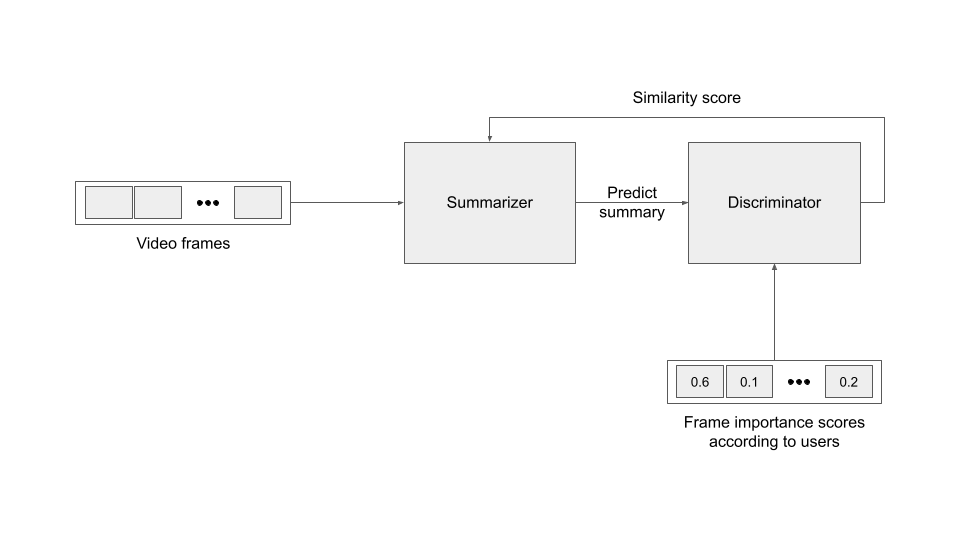
\includegraphics[width=0.73\paperwidth]{content/related/figures/sup-gan.png}
  \label{figure:rel-sup-gan}
\end{figure}

Taking a distinct approach to bridge the gap between machine-generated and ground-truth summaries, certain methods leverage Generative Adversarial Networks (GANs). Illustrated in \hyperref[figure:rel-sup-gan]{Figure \ref{figure:rel-sup-gan}}, the Summarizer, acting as the GAN's Generator, takes the video frames as input and generates a summary by computing frame-level importance scores. These predicted scores, along with an optimal video summary based on user preferences, are fed to a trainable Discriminator, which evaluates their similarity and outputs a corresponding score. The training process encompasses an adversarial framework where the Summarizer aims to deceive the Discriminator by producing summaries that are indistinguishable from the user-generated ones, while the Discriminator learns to differentiate between them. When the Discriminator's confidence level becomes low, indicating an equal classification error for both machine- and user-generated summaries, the Summarizer successfully generates summaries that align closely with users' expectations. Zhang \etal~\cite{zhang2019dtr} introduced a method that employs LSTMs and Dilated Temporal Relational (DTR) units to capture temporal dependencies across different time windows. Their approach trains the Summarizer by attempting to mislead a trainable discriminator into distinguishing between machine-generated summaries, ground-truth summaries, and randomly created summaries. Fu \etal~\cite{fu2019attentive} proposed an adversarial learning technique for (semi-)supervised video summarization, where the Generator/Summarizer is an attention-based Pointer Network. It determines the start and end points of each video fragment used in the summary. The Discriminator, a 3D-CNN classifier, determines whether a fragment belongs to a ground-truth or machine-generated summary. Instead of using a conventional adversarial loss, their algorithm employs the output of the Discriminator as a reward for training the Generator/Summarizer through reinforcement learning. While the use of GANs in supervised video summarization is relatively limited, this machine learning framework has been extensively employed in unsupervised video summarization, which will be discussed in the subsequent section.